\documentclass{amsart}
\usepackage{amsmath}
\usepackage{minted}
\usepackage{fancyvrb}
\usepackage{xcolor}
\usepackage{color}
\usepackage{listings}
\usepackage{graphicx}
\usepackage{subfig}
\newtheorem{theorem}{Theorem}[section]
\newtheorem{lemma}[theorem]{Lemma}

\theoremstyle{definition}
\newtheorem{definition}[theorem]{Definition}
\newtheorem{example}[theorem]{Example}
\newtheorem{xca}[theorem]{Exercise}

\theoremstyle{remark}
\newtheorem{remark}[theorem]{Remark}

\numberwithin{equation}{section}
\lstset{
	basicstyle=\small\ttfamily,
	columns=flexible,
	breaklines=true
}
\setminted[c]{
	frame=lines,
	framesep=2mm,
	baselinestretch=1,
	fontsize=\footnotesize,
	bgcolor=black,
	style=vim,
	linenos
}
\setlength{\textwidth}{\paperwidth}
\addtolength{\textwidth}{-1in}
\calclayout

\makeatletter
\g@addto@macro{\newpage}{\nointerlineskip}
\makeatother



\begin{document}
\vspace*{-80pt}

\title{IMDB Sentiment Analysis}

\author{Luo, Robin (260851506)}
\author{Rousseau, Marc-Andre  (260089646)}
\author{Xu Bide, (260711367)}

\date{\today}
\begin{abstract}
We used ML techniques including logistic regression, naive Bayes and support vector machines to process the data from a large dataset of reviews and train our software to be able to distinguish a favourable review from a negative one.  In addition to the three methods listed, we used TF-IDF, where the frequency of occurrence of the words within the document and the dataset are both taken into account to ascertain word importance.  Our model was submitted to a kaggle competition and we obtained a score of 0.91786 for the model using a linear SVM, tf-idf.  This is a significant improvement on the Naive Bayes classification method which has an accuracy of approximately 0.83 \end{abstract}
\maketitle
\section{Introduction}(5+sentences)
The ubiquity of social networks is no longer a budding phenomenon and is part of the reality in which we now find ourselves.  Many popular sites have included ways for users to share their opinions on a variety of topics and therefore the ability to mine through these posts and determine how users feel about the things being discussed is extremely useful for businesses.  Knowing that a user or group of users desire something or find it appealing creates a market of opportunity for companies in search of low risk opportunities to expand their business operations.  This is one of the most alluring aspects of machine learning.  While the discovery of many of the mathematical underpinnings of machine learning have been discovered for quite some time, it is the rise in computing power which has given us the ability to use these techniques in otherwise intractable situations.  For example gradient descent was invented by the prolific mathematician Augustin-Louis Cauchy in 1847.  For our project, we were given 12500 positive and 12500 negative reviews to train our algorithm and another 25000 to test our code and submit our best guess as to the correct labeling of the test reviews as either positive or negative.  Our best model which used a linear SVM (0.918 accuracy), was much better than Naive Bayes (0.83).
\section{Related Work}(4+sentences)
Machine learning and sentiment analysis are hot topics of research with many machine learning conferences having several talks on the topic.  For example, Twitter has been releasing datasets to be mined for things like whether a piece of task is positive, negative or neutral.  Recently, a group of researchers extended this problem to five classification categories and added arabic language content (Rosenthal, 2017).  Many teams submitted ML proposals to classify the twitter posts and the top performing groups used deep neural networks (DNNs) (Rosenthal, 2017).  In addition, out of the top 10 submissions, the second most successful approach to DNNs involved the use of SVMs which is consistent with our best performing model for this project.  A more directly related work involved taking into account sentence negations (Das, 2018).  In this paper, the authors have decided to use a shortcut for negation by negating the word immediately following a negation.  One example of this method would be to take the sentence "I am not happy" which gets converted to "I am not\_happy".  The benefit of this is that by changing only one word, they are able to change the meaning of the entire sentence (Das, 2018).  Our team implemented this feature but it did not have a significant impact on the score as checked by the cross-validation.
\section{Dataset and Setup}(3+sentences)
Our training dataset consisted of a list of 25000 reviews properly marked as positive or negative for us to train.  We also had another 25000 data points to test out our model.  The data consist of the content of the reviews and both the training and test sets needed to have their data preprocessed to be able to be consumed by the python libraries.  For the purpose of training and validation, we separated our data into 80\% training and 20\% validation.
\section{Proposed Approach}(7+sentences)
\subsection{Preprocessing}
For the preprocessing, we considered several models including a raw text input model, a model where the text was cleaned to only include letter characters (LC), a model where the text was processed through a normalization library and the words were separated from the punctuation symbols (SWP), a model with lemmatization (LZ) and a model with next word negation (NWN) from the previously mentioned paper.  For the model where the text input was cleaned and normalized, we also converted the text to lowercase.  Following the initial preprocessing, the data was subsequently tokenized.  For the normalization model, we removed any characters for which the normalization library could not process.  This was usually due to unicode characters which could not be mapped to equivalent ascii characters.
\subsection{Feature, hyperparamter and model selection}
In addition to the features generated by the preprocessing, we used tf-idf and bag of words (BOW) in our pipelines for feature selection.  While we eventually submitted an SVM model as our final model, we also implemented Laplace-smoothed Bernoulli Naive Bayes (NB) and logistic regression (LR) models.  To determine the hyperparameters and for regularization as well as the feature selection, we used a grid-based search algorithm with a cross-validation parameter of 5.  For our BOW feature, we tested out many different values for possible n-gram size and settled with 1-4 after testing out several different options.  For the SVM model, we tried values for the penalty parameter "c" and decided to use the default value of 1.  In addition to this, once our model was able to associate good or bad to a particular set of words, we used these word to sentiment mappings to analyse subsentences separated by punctuation.  For each bad or good word found, we added 1 or -1 to a counter and then classified the value for the overall text to the sum of all the individual good/bad words found in the text.  In addition to this, we used a normalization library to standardize the feature vectors so that they had unit length.  In terms of the theoretical underpinnings of the model selection, we used a data-driven approach rather than a conceptual one and so there was little discussion about which model was more appropriate and instead we opted to go with the model that had the best predictive power.

\section{Results}
The task of deciding on a final model based on the performance is quite easy since we only had to code the model and then pick whichever model worked the best, however a discussion of the relative performance of the models is difficult due to how close the top models performed as well as the sheer quantity of possible adjustments.  In general, tf-idf outperformed bag of words, SVM outperformed LR and a model allowing for tetragrams outperformed the trigram models.
\subsection{NB vs LR vs SVM}
The performance of the Naive Bayes was significantly better than a random guess approach but still failed to come close to the performance of the logistic regression or the support vector machine approaches.  One of the fundamental differences between our implementation of Naive Bayes and the other two models is that the former does not exclude words whereas the other two had minimum cutoffs for features.  This could account for the performance difference seen between the bag of words LR and the Naive Bayes model.  Our top performing model on cross-validation was a LR model but this did not extend to kaggle submissions for which the SVM slightly outperformed the LR.
 \subsection{Bag of words vs tf-idf}
The performance of SVM and LR using both BOW and TF-IDF were similar with TF-IDF being slightly better than BOW according to the parameters we chose for min-df and max-df.  For our model, we used a min\_df of 2 and a max\_df of 1 meaning that words that appeared in at least 2 of the documents were considered and no constraint was placed on the maximum frequency that a word could occur.  In addition to using these models, we had originally also included stop\_words but these did not show any additional gains above and beyond tf-idf and therefore it would seem as though the idf aspect of the tf-idf implementation may have already been incorporating the information contained in stop\_words by essentially removing those words which were used too frequently by lowering the respective weights.  Looking at the values in Table 1, we can see that for models where BOW and TF-IDF were used, the latter usually performed slightly better.  A strict comparison of these features is difficult due to the many possible parametrizations of the BOW implementation.  Figure 1 shows how the max\_df affects the score and the difference in the score between the BOW and tf-idf be partially due to the inclusion of those common words which appear in almost every paragraph of english ("in","the", etc...).
\begin{figure}
	\centering
	\subfloat[score vs max\_df]{{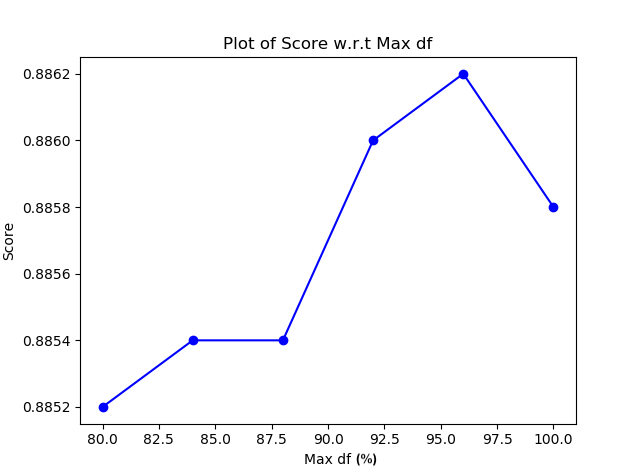
\includegraphics[width=5cm]{fig/max_df_score1.png} }}
	\qquad
	\subfloat[total runtime vs max\_df]{{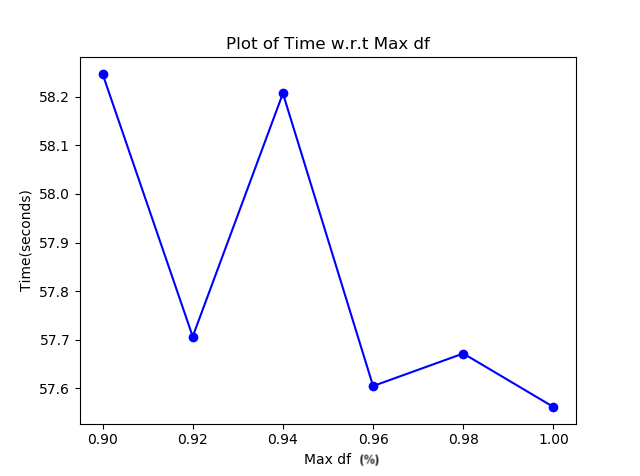
\includegraphics[width=5cm]{fig/max_df_time1.png} }}
	\caption{\textbf{Performance analysis of the max\_df parameter}  In A,  we can see the best prediction is obtained just shy of the 100 percent mark which might account for why our BOW model did slightly worse than the tf\_idf model which would automatically account for the high frequency words.  In (B), we see that above the 90 percent mark, there is little effect on the runtime which coud simply be due to the fact that there are few words which appear extremely frequently and therefore there is no discernable effect on runtime}
	\label{fig:betavsMSE}
\end{figure}
\subsection{N-grams}
We considered many different possibilities for n-grams but ultimately we settled on using (1-4)-grams even though the gain in performance was quite small between limiting ourselves to trigrams and including tetragrams.  The logistic regression model with td-idf showed that the value in increasing above tetragrams was nonexistent.  While the increase in score between the trigram and tetragram models was under 1 percent for most models, the increase seemed consistent across almost all models considered and therefore we included it.  The additional value added by going to a fourth level of n-gram is probably due to common expressions in the english language which convey sentiment.  The low increase in performance is quite simply due to the low frequency of occurrence of these expressions overall for the amount of data we had.
\subsection{Text processing}
The effect of processing and preparing the text was a contributor to performance as can be seen by comparing the values in Table 1.  We can see that by limiting ourselves to letters exclusively, we actually lose some information and the score for the LC models suffered as a result.  As an example, the model using LR, tf-idf and (1-4)-grams had a performance score of 0.895 for the letter character model, a score of 0.913 for the raw text and 0.915 for the model where the text was normalized and converted to lowercase.  The increase in performance between the raw and cleaned data was not universally consistent which could be due to the cleaning removing some information that would otherwise have been useful.  One of the most interesting results is that some of the numbers actually ranked quite high in the tf-idf
\subsection{Lemmatization}
The lemmatization seemed to perform consistently better than a non-lemmatized model but the extension to the kaggle dataset suggested that there was in fact a gain in performance in using the lemmatized model.  Lemmatization is a feature which reduces the information rather than increases it and therefore it is not surprising to see some drop in perfomance.  Despite this, the idea behind lemmatization is that there are many words for which only the root of the word conveys information and therefore this should help reduce noise and regularize so as to better extend our model to unseen data.
\subsection{SWP and NWN}
The SWP and NWN models did not seem to provide significant improvements to our model after having already incorporated tf-idf, lemmatize, and a cleaning of the text.  While it is true that our best performing model used SWP (Table 1), this result did not extend into the kaggle submission and could be due to random variance in the data.  We had expected some gain in performance from the NWN and had also tried other forms of regularization of negation but no clear improvement was seen in our kaggle submissions or our cross-validation.  
\subsection{Conclusion}

\section{Division of Work}
\begin{itemize}
\item{\textbf{Robin Luo}}: Model fitting 
\item{\textbf{Marc-Andre Rousseau}}: Literature research, TeXing, some minor coding.
\item{\textbf{Peter Xu}}: Coding, feature selection and hyperparameter fitting.
\end{itemize}
\section{References}
\begin{itemize}
	\item [1] Rosenthal, Sara, et al. “SemEval-2017 task 4: Sentiment analysis in Twitter” Proceedings of the 11th International Workshop on Semantic Evaluations (SemEval-2017), pp. 502–518.
	\item [2] Das, Bijoyan. Chakraborty, Sarit. "An improved text sentiment classification model using tf-idf and next word negation" June, 2017, eprint arXiv:1806.06407
\end{itemize}
\section{Appendix}
\begin{center}
	\begin{table}
		\caption{Runtime and F1 performance analysis of various models} \label{tab:title}
		\begin{tabular}{|| c | c | c | c | c ||}
			\hline
			Model & F1-score & \#features & Fit runtime (s) & Prediction runtime (s) \\
			\hline\hline
			Bernoulli NB + BOW & 0.84879 & 67708 & 1020 & 5520 \\
			\hline
			LR,LCs, 1-gram & 0.88561 & 27254 & 10 & 2 \\
			\hline
			LR, BOW, LCs, (1-4)-gram &  0.88961 & 104211 & 106 & 7 \\
			\hline
			LR, tf-idf, LCs, (1-4)-gram & 0.89481 & 104211 & 95 & 6 \\
			\hline
			LR, tf-idf, raw, 1-gram & 0.88541 & 27745 & 29 & 4 \\
			\hline
			LR, BOW, raw, (1-2)-gram & 0.89521 & 166041 & 54 & 9 \\
			\hline
			LR, BOW, raw, (1-3)-gram & 0.89601 & 290118 & 114 & 14 \\
			\hline
			LR, BOW, raw, (1-4)-gram & 0.89521 & 342886 & 230 & 230 \\
			\hline
			LR, tf-idf, raw, 1-gram & 0.89181 & 27745 & 20 & 6 \\
			\hline
			LR, tf-idf, raw, (1-2)-gram & 0.90881 & 166041 & 55 & 8 \\
			\hline
			LR, tf-idf, raw, (1-3)-gram & 0.91161 & 290118 & 110 & 10 \\
			\hline
			LR, tf-idf, raw, (1-4)-gram & 0.91301 & 342886 & 199 & 20 \\
			\hline
			LR, tf-idf, raw, (1-5)-gram & 0.91301 & 358250 & 211 & 13 \\
			\hline
			LR, tf-idf, cleanup, (1-3)-gram & 0.91381 & 284493 & 116 & 12 \\
			\hline
			LR, tf-idf, cleanup, (1-4)-gram & 0.91581 & 334013 & 169 & 18\\
			\hline
			LR, tf-idf, cleanup, SWP, (1-3)-gram & 0.91441 & 284955 & 117 & 10 \\
			\hline
			\textbf{LR, tf-idf, cleanup, SWP, (1-4)-gram} & \textbf{0.91561} & \textbf{333673} & \textbf{166} & \textbf{20} \\
			\hline
			LR, tf-idf, cleanup, lemmatize, (1-3)-gram & 0.91161 & 283063 & 108 & 11\\
			\hline
			LR, tf-idf, cleanup, lemmatize, (1-4)-gram & 0.91281 & 334089 & 178 & 12 \\
			\hline
			LR, tf-idf, cleanup, NWN, (1-3)-gram & 0.91381 & 264522 & 89 & 9\\
			\hline
			LR, tf-idf, cleanup, NWN, (1-4)-gram & 0.91441 & 297461 & 147 & 11\\
			\hline
			LR, tf-idf, cleanup, Lemmatize, SWP (1-3)-gram & 0.91201 & 283682 & 85 & 8 \\
			\hline
			LR, tf-idf, cleanup, Lemmatize, SWP (1-4)-gram & 0.91241 & 333997 & 141 & 11\\
			\hline
			LR, tf-idf, cleanup, Lemmatize, SWP, NWN, (1-3)-gram & 0.91281 & 263993 & 90 & 9 \\
			\hline
			LR, tf-idf, cleanup, Lemmatize, SWP, NWN, (1-4)-gram & 0.91261 & 298356 & 132 & 10\\
			\hline
			SVM, tf-idf, raw, (1-4)-gram & 0.91521 & 1010594 & 167 & 13 \\
			\hline
			SVM, tf-idf, cleanup, (1-4)-gram & 0.91501 & 987640 & 155 & 15 \\
			\hline
			SVM, tf-idf, cleanup, NWN, (1-4)-gram & 0.91401 & 899187 & 156 & 12\\
			\hline
			\textbf{SVM, tf-idf, cleanup, Lemmatize, (1-4)-gram} & \textbf{0.91321} & \textbf{987519} & \textbf{171} & \textbf{12}\\
			\hline
			SVM, tf-idf, cleanup, SWP, (1-4)-gram & 0.91481 & 988012 & 161 & 16\\
			\hline
			SVM, tf-idf, cleanup, SWP, Lemmatize, NWN, (1-4)-gram & 0.91541 & 901848 & 164 & 13\\
			\hline\hline
		\end{tabular}
		\caption*{\textbf{Summary of selected models considered for our final submission.} The final model performance was determined via a study of the effect of modifying the parameters on the F1-scores.  All runtimes with the exception of the Naive Bayes did not preclude extensive testing.  A subset of the models under consideration have been presented.  Our best performing model on the cross validation as well as the best performing model on kaggle are in bold.}
	\end{table}
\end{center}
\end{document}
